\documentclass{article}

\usepackage[utf8]{inputenc}
\usepackage[french]{babel}

\usepackage[a3paper,margin=1in,landscape]{geometry}

\usepackage[table]{xcolor}
\definecolor{lightgray}{gray}{0.94}
\let\oldtabular\tabular
\let\endoldtabular\endtabular
\renewenvironment{tabular}{\rowcolors{1}{lightgray}{white}\oldtabular}{\endoldtabular}

\usepackage{comment}

\usepackage{multicol}
\setlength{\columnsep}{0.5cm}
\usepackage{wrapfig}

\usepackage{graphicx}

\usepackage{hyperref}
\hypersetup{
colorlinks=true,
linkcolor=blue,
urlcolor=blue,
}

\usepackage{fancyhdr}
\pagestyle{fancy}
\fancyhead[C]{{\huge \textbf{Fudge en une page}}}

\fancyfoot{}
\renewcommand{\headrulewidth}{0.4pt}
\renewcommand{\footrulewidth}{0.4pt}



% Mes macros

\newcommand{\mysection}[1]{
\vspace{0.2cm}
\noindent{\large \textbf{#1}}
}

\newcommand{\mysubsection}[1]{
\vspace{0.1cm}
\noindent{\textit{\textbf{#1}}}
}


%=======================================DOC
\begin{document}

\begin{multicols*}{3}

Bien que Fudge soit conçu pour être adapté par chaque Maître de Jeu (MJ), certains éléments de conception du jeu au cœur de Fudge sont utilisés par la plupart des MJ.

\mysection{Personnages et Traits}

Les personnages de Fudge sont définis par des \textit{Traits}, incluant des \textit{Caractéristiques} (tout trait que tout le monde possède dans l’univers de jeu), des \textit{Compétences} (tout trait qui n'est pas une caractéristique et qui peut être amélioré par la pratique), des \textit{Dons} (tout trait qui n'est ni une caractéristique, ni une compétence, mais qui est quelque chose de positif pour le personnage), et des \textit{Défauts} (tout trait qui limite les actions du personnage, ou qui implique des réactions négatives de la part des autres personnes). Les \textit{Pouvoirs Surnaturels} sont traités comme des Dons puissants.

\begin{wraptable}{l}{0.43\linewidth}
\begin{tabular}{ccc}
+3 & Fantastique & Superb \\
+2 & Excellent & Great \\
+1 & Bon & Good \\
0 & Correct & Fair \\
-1 & Médiocre & Mediocre \\
-2 & Mauvais & Poor \\
-3 & Lamentable & Terrible \\
\end{tabular}
\end{wraptable}

Fudge emploie des mots ordinaires pour décrire certains Traits, en particulier les Caractéristiques et les Compétences. La liste des termes suivants, arrangés dans une séquence à sept degrés, sont les mots suggérés par l'auteur de Fudge et utilisés dans les produits Grey Ghost Games.

Il existe un niveau additionnel non listé ci-dessus : Légendaire, qui se situe au delà de Fantastique. Les MJs peuvent restreindre les traits Légendaires aux Personnages Non Joueurs (PNJ).

Il n’y a pas de liste figée de Traits, chaque MJ peut la définir à loisir. De nombreux exemples sont donnés dans le Manuel.

\mysection{Création des personnages}

Fudge propose deux façons basiques de créer des personnages : le système "subjectif" et le système "objectif".

Dans le système subjectif, le joueur et le MJ travaillent ensemble pour définir le personnage dans les termes utilisés par Fudge, en commençant par un concept solide pour le personnage. Dans le système objectif, les Traits d'un personnage démarrent à un niveau par défaut (Correct pour les caractéristiques, Mauvais pour les compétences) et le MJ accorde aux joueurs un nombre de niveaux gratuits à allouer. Le MJ peut aussi accorder des Dons gratuits, ou demander de choisir un ou plusieurs Défauts.

Le joueur peut alors, par exemple, dépenser deux niveaux pour passer une caractéristique de Correcte à Excellente ; ou sacrifier un nombre de niveaux pour gagner un Don ; ou choisir un Défaut pour son personnage de façon à gagner des niveaux à répartir autre part.

Les valeurs d'échange des différents traits en termes de niveaux sont :


\begin{center}\begin{tabular}{ccc}
1 niveau de Caractéristique & = & 3 niveaux de Compétences \\
1 Don & = & 6 niveaux de Compétences \\
1 Don & = & 2 niveaux de Caractéristiques \\
1 Don & = & 1 Défaut \\
\end{tabular}\end{center}

\mysection{Echelle -- Force et Masse}

Certains personnages et créatures ont des caractéristiques qui sont très au delà de la norme humaine. Les premier exemples concernent la Force, la Masse et la Vitesse. Ces caractéristiques sont notées sur une Echelle, qui agit comme un modificateur pour les interactions entre créatures ou objets de différentes tailles.

Dans un jeu centré sur les humains, l'Echelle humaine est de 0. Une race ayant une force surhumaine pourrait être sur l'Echelle de Force +1 ou plus, tandis qu'une race de Force moindre que la Force moyenne humaine serait sur l'Echelle de Force -1 ou moins. De ce fait, les individus qui ont une Force Correcte ou de Bon niveau, l'ont relativement à leur Echelle.

Dans un jeu où les joueurs incarnent des lapins, L'Echelle des lapins serait l'échelle 0, tandis que l'échelle humaine serait probablement +7. Dans un jeu "Mecha" où les joueurs incarnent des robots géants, l'Echelle Mecha serait de 0 et l'échelle humaine dépendrait du rapport de taille entre les Mechs et les humains, probablement -15.

Pour calculer les valeurs appropriées d'Echelle de Force/Masse, il faut comprendre que chaque niveau N d'échelle de Force est de 1,5 fois supérieur à l'Echelle de Force/Masse du niveau N-1. Cela est dû au fait que les règles de base de Fudge définissent chaque niveau de Force comme étant 1,5 fois plus fort que le niveau du dessous.

Cette progression n'est pas forcément la même avec toutes les caractéristiques. Une Dextérité Fantastique est seulement deux fois plus grande qu'une Dextérité Correcte, en raison du fait que chaque niveau de Vitesse est 1,2 fois le niveaux du dessous.

Il est important de noter qu'un niveau de Force Correcte sur l'Echelle 1 n'est pas tout à fait égal à un Bon niveau de Force sur l'Echelle 0 : l'Echelle Force/Masse mesure aussi la Masse et la densité et joue sur la facilité de causer des dommages à une créature. Le guerrier d'Echelle 1 est moins affecté par les blessures en raison de sa plus grande Masse.

\mysection{Résolution des actions}

Pour chaque action que le personne souhaite effectuer, le MJ doit déterminer quel Trait est testé (c'est généralement une Caractéristique ou une Compétence). Si l'action est sans opposition, le MJ détermine le niveau de difficulté. Certaines actions sont si faciles que le personne réussit automatiquement ; d'autres sont impossibles (pas de jet de dés).

\mysubsection{Actions sans opposition}

Chaque action que le personnage effectue sans être influencé par quiconque est dénommé action sans opposition, par exemple sauter au dessus d'un gouffre béant, escalader une falaise, etc.

\textit{Niveau de difficulté} : le MJ déterminera un niveau de difficulté quand un personnage tentera une action sans opposition. Normalement, le niveau de difficulté est Correct, mais certaines tâches sont plus faciles ou plus difficiles.

\textit{Degré de réussite} : Ce terme se réfère au niveau de réussite du personnage pour une certaine tâche. Si quelqu'un est Bon en escalade et qu'il tire un +1 au jet de dés, alors le degré de réussite sera un niveau de plus que son niveau, soit Excellent. Les degrés de réussite Fantastique +1 à Fantastique +4 étant possibles, le MJ pourra déterminer un niveau de difficulté au delà de Fantastique pour les actions presqu'impossibles. De la même façon, il existe des degrés de réussite de Lamentable -1 à Lamentable -4. Le MJ devrait utiliser son imagination pour déterminer les conséquences d'échecs aussi abyssaux.

\mysubsection{Actions en opposition}

Les actions sont en opposition quand quelqu'un d'autre (ou des animaux, etc.) peuvent avoir un effet dans le résultat de l'action. Dans ce cas, le joueur jouant chaque adversaire jette des dés, et les résultats sont comparés pour déterminer le résultat.

\textit{Degré relatif} : ce terme se réfère au niveau de réussite d'un personnage en comparaison du niveau de l'autre participant à l'action en opposition. Le niveau relatif est exprimé en nombre de niveaux. Si un PJ obtient un Bon niveau dans un combat, et que le PNJ antagoniste obtient un Médiocre, le PJ bat son adversaire de 2 niveaux, +2 vu du PJ et -2 vu du PNJ.

\mysection{Dés Fudge}

Les dés Fudge sont des dés à 6 faces avec deux faces marquées + (+1), deux faces marquées - (-1) et deux faces laissées blanches (+/-0).Lancer quatre dés Fudge (4dF) donne un résultant allant de -4 (potentiellement sous Lamentable) à +4 (encore mieux que Fantastique). Pour déterminer le résultat d'une action, lancer les dés ; utilisez le résultat pour modifier le Trait qui est en train d'être testé. Par exemple, un résultat +3 ajouté à un Trait Correct est un degré de réussite Fantastique ; un -1 ajouté à un Trait Correct indique un résultat Médiocre. 

\mysection{Blessures}

Les dommages subis par un personnage peuvent être décrits comme faisant partie d'un des sept états de sévérité :

\begin{center}\begin{tabular}{cc>{\centering\arraybackslash}p{5cm}}
Pas de dommages & = & Pas de blessures du tout \\
Juste une égratignure & = & Pas d'effet réel dans le jeu \\
Blessé & = & -1 sur tous les Traits \\
Gravement blessé & = & -2 sur tous les Traits \\
Immobilisé & = & Seules les actions les plus basiques sont autorisées \\
Mort imminente & = & Inconscient, mort si pas d'aide médicale \\
\multicolumn{3}{c}{Mort} \\
\end{tabular}\end{center}

\textit{Déterminer les niveaux de blessure} : Fudge offre plusieurs façon de suivre les dommages résultants des combats. Le Système de Dommages Objectif suppose que chaque personnage possède un Facteur de Dommages Offensifs (le total des modificateurs, incluant tous les bonus de Force et d'Echelle, qui illustrent la létalité de l'arme utilisée) et un Facteur de Dommages Défensif (le total des modificateurs, incluant l'Echelle et l'armure, qui reflète la capacité du personnage à encaisser ou éviter les dommages).

Pour déterminer combien de dommages sont créés durant un round de combat, la formule suivante peut être utilisée :

\begin{center}\textbf{Degré relatif du vainqueur + Facteur de Dommages Offensif - Facteur de Dommages Défensif du perdant}\end{center}

\begin{center}\begin{tabular}{lccccc}
Dommage: & 1-2 & 3-4 & 5-6 & 7-8 & 9+ \\
Blessures: & Egrat. & Blessé & Grav. blessé & Immob. & Mort Imm. \\
\end{tabular}\end{center}

La plupart des personnages peuvent supporter 3 Egratignures, une Blessure et une Blessure Grave. Une nouvelle égratignure est marquée comme Blessure, une nouvelle Blessure est marquée comme Blessure Grave, etc. Pour un jeu plus cinématographique, les MJ peuvent ajuster les cases Blessure, autorisant deux Blessures à la place d'une seule, par exemple.

Pour en savoir plus sur Fudge, consultez \href{https://www.fudgerpg.com}{www.fudgerpg.com}.

\begin{center}
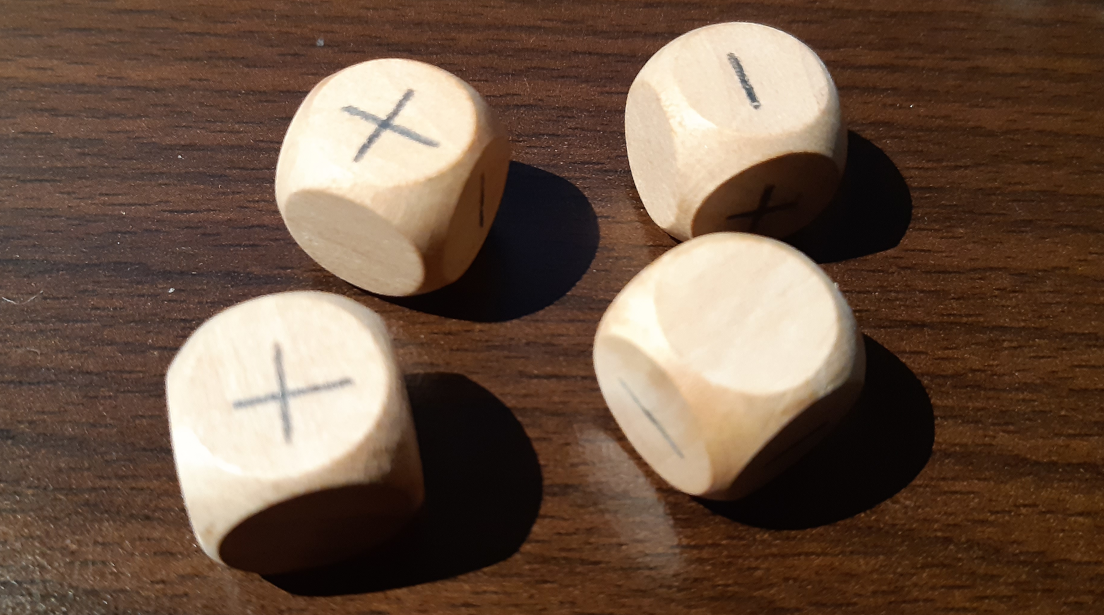
\includegraphics[scale=0.15]{4dF}
\end{center}

\mysection{Licence}

Fudge est un jeu de rôles écrit par Steffan O’Sullivan, avec la contribution importante de la communauté usenet de \textit{rec.games.design} et d'autres forums en ligne. Les règles de base de Fudge sont disponibles gratuitement sur Internet sur \href{https://www.fudgerpg.com}{www.fudgerpg.com} et sur d'autres sites. Fudge a été conçu pour être customisé, et il peut être utilisé avec n'importe quel genre de jeu. Les maîtres de jeu Fudge et les concepteurs de jeux sont encouragés à modifier Fudge pour coller à leurs besoins, et à partager leurs modifications et additions avec la communauté Fudge.

Le système de jeu Fudge est sous copyright ©2000, 2005 par Grey Ghost Press, Inc., et est disponible sous la licence \href{https://web.archive.org/web/20160302062643/http://www.wizards.com/d20/files/OGLv1.0a.rtf}{Open Game License 1.0a}. Voir le site fudgerpg.com pour plus d'information.
\end{multicols*}



\end{document}
